\documentclass[a4paper,12pt]{report}

% Packages nécessaires
\usepackage[utf8]{inputenc}
\usepackage[T1]{fontenc}
\usepackage[french]{babel}
\usepackage{graphicx}
\usepackage{amsmath, amssymb}
\usepackage{hyperref}
\usepackage{geometry}
\usepackage{listings}
\usepackage{xcolor}
\usepackage{float}
\usepackage{caption}
\usepackage{subcaption}

% Configuration de la mise en page
\geometry{hmargin=2.5cm,vmargin=2.5cm}

% Configuration pour l'affichage du code
\definecolor{codegreen}{rgb}{0,0.6,0}
\definecolor{codegray}{rgb}{0.5,0.5,0.5}
\definecolor{codepurple}{rgb}{0.58,0,0.82}
\definecolor{backcolour}{rgb}{0.95,0.95,0.92}

\lstdefinestyle{mystyle}{
    backgroundcolor=\color{backcolour},   
    commentstyle=\color{codegreen},
    keywordstyle=\color{magenta},
    numberstyle=\tiny\color{codegray},
    stringstyle=\color{codepurple},
    basicstyle=\ttfamily\footnotesize,
    breakatwhitespace=false,         
    breaklines=true,                 
    captionpos=b,                    
    keepspaces=true,                 
    numbers=left,                    
    numbersep=5pt,                  
    showspaces=false,                
    showstringspaces=false,
    showtabs=false,                  
    tabsize=2
}

\lstset{style=mystyle}

% Informations du document
\title{\textbf{Implémentation et Analyse de la Méthode SIFT}\\ (Scale-Invariant Feature Transform)}
\author{Louis LENOBLE, Raphael ROGER, Dylan SANSON, Jack SU \\ \\ \textit{Projet TIM - Traitement d'Image}}
\date{28 Novembre 2025}

\begin{document}

\maketitle

\begin{abstract}
Ce rapport présente une étude approfondie et une implémentation de l'algorithme SIFT (Scale-Invariant Feature Transform), initialement proposé par David G. Lowe en 2004. SIFT est une méthode robuste pour l'extraction de caractéristiques locales dans les images, invariante aux changements d'échelle, à la rotation et partiellement invariante aux changements d'illumination et au point de vue 3D. Nous détaillons les quatre étapes fondamentales de l'algorithme : la détection des extrerums dans l'espace des échelles, la localisation précise des points clés, l'assignation d'orientation et la création des descripteurs. Nous présentons ensuite notre propre implémentation en Python, en analysant les choix techniques effectués. Enfin, nous discutons des applications possibles (telles que le stitching d'images et la réalité augmentée) ainsi que des limites intrinsèques de la méthode.
\end{abstract}

\tableofcontents

\chapter{Introduction}

La vision par ordinateur a pour but ultime de permettre aux machines de comprendre et d'interpréter le monde visuel. Au cœur de nombreux systèmes de vision moderne — qu'il s'agisse de la reconnaissance d'objets, de la reconstruction 3D, de la création de panoramas (stitching) ou de la navigation robotique — se trouve un problème fondamental : la mise en correspondance d'images (\textit{image matching}).

Pour identifier qu'un objet présent dans une image A est le même que celui dans une image B, l'algorithme doit être capable d'identifier des points d'intérêt communs, malgré les transformations drastiques que l'image a pu subir entre les deux prises de vue.

\section{Contexte et Problématique}

Les images du monde réel sont soumises à de nombreuses variations qui rendent la comparaison pixel par pixel impossible. Un système de reconnaissance robuste doit être capable de gérer :
\begin{itemize}
    \item \textbf{Les changements d'échelle :} L'objet peut être proche ou lointain.
    \item \textbf{Les rotations :} L'objet ou la caméra peuvent avoir tourné.
    \item \textbf{Les changements d'illumination :} La lumière peut varier en intensité ou en direction.
    \item \textbf{Le point de vue 3D :} Une perspective différente déforme l'apparence 2D de l'objet (distorsion affine).
    \item \textbf{Le bruit et les occultations :} L'image peut être dégradée ou l'objet partiellement caché.
\end{itemize}

L'objectif est donc d'extraire des "caractéristiques" (\textit{features}) locales qui sont invariantes à ces transformations. Ces caractéristiques doivent être suffisamment distinctives pour ne pas être confondues avec d'autres points de l'image.

\section{Limites des Approches Historiques}

Avant l'avènement de SIFT, les méthodes de détection de points d'intérêt se basaient principalement sur la détection de coins (\textit{corners}). L'algorithme le plus célèbre, le détecteur de Harris-Stephens (1988), identifie les régions où l'intensité de l'image change significativement dans toutes les directions.

Bien que le détecteur de Harris soit très efficace pour l'invariance en rotation (un coin reste un coin même si l'image tourne), il souffre d'une limitation majeure : il n'est pas invariant à l'échelle.
\begin{figure}[h]
    \centering
    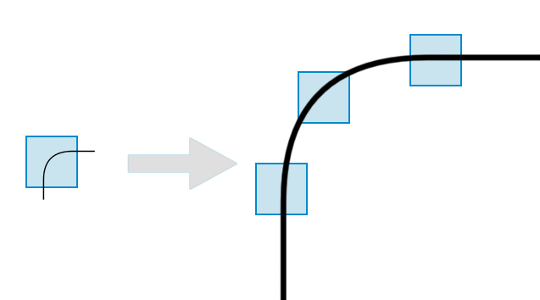
\includegraphics[width=0.8\textwidth]{img/harris_limites.png}
    \caption{\textit{Illustration du problème d'invariance d'échelle avec le détecteur de Harris. Les coins détectés à une échelle ne sont pas retrouvés à une autre échelle. Extrait de Lowe, D. G. (2004). Distinctive Image Features from Scale-Invariant Keypoints.
International Journal of Computer Vision.}}
    \label{fig:harris_issue}
\end{figure}

Comme nous l'avons souligné dans notre présentation, pour repérer des coins à différentes échelles avec Harris, il faudrait adapter manuellement la taille de la fenêtre de détection, ce qui est une tâche fastidieuse et peu robuste pour une automatisation complète.

\section{La Proposition SIFT}

C'est dans ce contexte que David G. Lowe a proposé, dans son papier fondateur de 2004 \textit{"Distinctive Image Features from Scale-Invariant Keypoints"}, la méthode SIFT (Scale-Invariant Feature Transform).

L'idée révolutionnaire de SIFT est de ne pas analyser l'image à une seule résolution, mais de construire un \textbf{espace des échelles} (\textit{scale-space}). En recherchant des extremums stables à travers toutes les échelles possibles, SIFT permet d'identifier des points d'intérêt qui sont intrinsèquement liés à la taille des structures de l'image.

Selon Lowe, les caractéristiques SIFT possèdent des propriétés remarquables :
\begin{enumerate}
    \item \textbf{Invariance :} Elles sont invariantes à l'échelle et à la rotation, et font preuve d'une grande robustesse face aux changements d'illumination et au bruit.
    \item \textbf{Distinctivité :} Chaque point clé est associé à un descripteur riche (vecteur de 128 dimensions) qui permet de le différencier avec une très haute probabilité parmi une grande base de données de features.
    \item \textbf{Quantité :} La méthode génère un grand nombre de features (même sur de petits objets), ce qui augmente la fiabilité de la reconnaissance, même en cas d'occultation partielle.
\end{enumerate}

\section{Objectifs du Rapport}

Ce rapport a pour but de décortiquer le fonctionnement de cet algorithme emblématique. Notre démarche s'articule autour de trois axes :
\begin{enumerate}
    \item \textbf{Compréhension Théorique :} Analyser les fondements mathématiques décrits par Lowe (Différence de Gaussiennes, développement de Taylor, histogrammes de gradients).
    \item \textbf{Implémentation Pratique :} Recréer l'algorithme SIFT "from scratch" en Python. L'objectif n'est pas d'utiliser la fonction toute faite `cv2.SIFT` d'OpenCV, mais de réécrire la logique de construction des octaves, de localisation des extremums et de création des descripteurs pour maîtriser les concepts sous-jacents.
    \item \textbf{Expérimentation :} Tester notre implémentation sur des images standards (comme "Box" ou "Cameraman"), visualiser les résultats (orientation, échelle) et discuter des limites rencontrées lors du développement.
\end{enumerate}

\chapter{Théorie de la méthode SIFT}

L'approche de SIFT décrite par David G. Lowe se décompose en quatre étapes séquentielles :
\begin{enumerate}
    \item \textbf{Détection des extremums dans l'espace des échelles :} Recherche initiale des points d'intérêt sur toutes les échelles et positions possibles.
    \item \textbf{Localisation des points clés :} Raffinement précis de la position et suppression des points instables (faible contraste ou situés sur des arêtes).
    \item \textbf{Assignation d'orientation :} Attribution d'une ou plusieurs orientations basées sur le gradient local pour assurer l'invariance par rotation.
    \item \textbf{Descripteur de point clé :} Création d'une signature vectorielle unique représentant le voisinage du point.
\end{enumerate}

\section{Détection des extremums dans l'espace des échelles}

La première difficulté de la vision par ordinateur est de repérer le même objet à différentes distances. Un "coin" net à une certaine distance peut devenir une tache floue s'il est vu de loin. Pour résoudre ce problème, SIFT recherche des structures stables à travers un \textit{espace des échelles} continu.

\subsection{Espace des échelles et convolution Gaussienne}
L'espace des échelles d'une image est une fonction $L(x,y,\sigma)$ obtenue par la convolution de l'image originale $I(x,y)$ avec un noyau Gaussien $G(x,y,\sigma)$ de largeur variable $\sigma$ :

\begin{equation}
    L(x,y,\sigma) = G(x,y,\sigma) * I(x,y)
\end{equation}

où $G(x,y,\sigma) = \frac{1}{2\pi\sigma^2}e^{-(x^2+y^2)/2\sigma^2}$. Plus $\sigma$ est grand, plus l'image est floutée, simulant une observation de l'objet à une plus grande distance (perte des détails haute fréquence).

\subsection{Différence de Gaussiennes (DoG)}
Pour détecter des points d'intérêt caractéristiques (comme des taches ou des coins), on cherche traditionnellement les extremums du Laplacien de Gaussienne ($\sigma^2 \nabla^2 G$). Cependant, cette opération est coûteuse en calcul.
Lowe propose d'approximer ce Laplacien par une \textbf{Différence de Gaussiennes} (DoG), notée $D(x,y,\sigma)$, qui est beaucoup plus rapide à calculer :

\begin{equation}
    D(x,y,\sigma) = L(x,y,k\sigma) - L(x,y,\sigma)
\end{equation}

\subsection{Organisation en Octaves}
Pour couvrir efficacement l'ensemble des échelles possibles, l'espace des échelles est discretisé en \textbf{octaves}.
\begin{itemize}
    \item Une octave correspond à un doublement de la valeur de $\sigma$.
    \item Chaque octave est divisée en $s$ intervalles (ou sous-niveaux) entiers.
\end{itemize}

Pour détecter des extremums dans $s$ intervalles, nous avons besoin de calculer les différences DoG. Pour obtenir $s$ images DoG, nous devons générer $s+1$ images DoG, et donc disposer de $s+3$ images gaussiennes ($L$) par octave.
Une fois une octave traitée, l'image gaussienne située à $2\sigma$ est sous-échantillonnée par un facteur 2 (un pixel sur deux est gardé) pour servir d'image de base à l'octave suivante. Cela réduit considérablement la complexité algorithmique.

\begin{figure}[h]
    \centering
    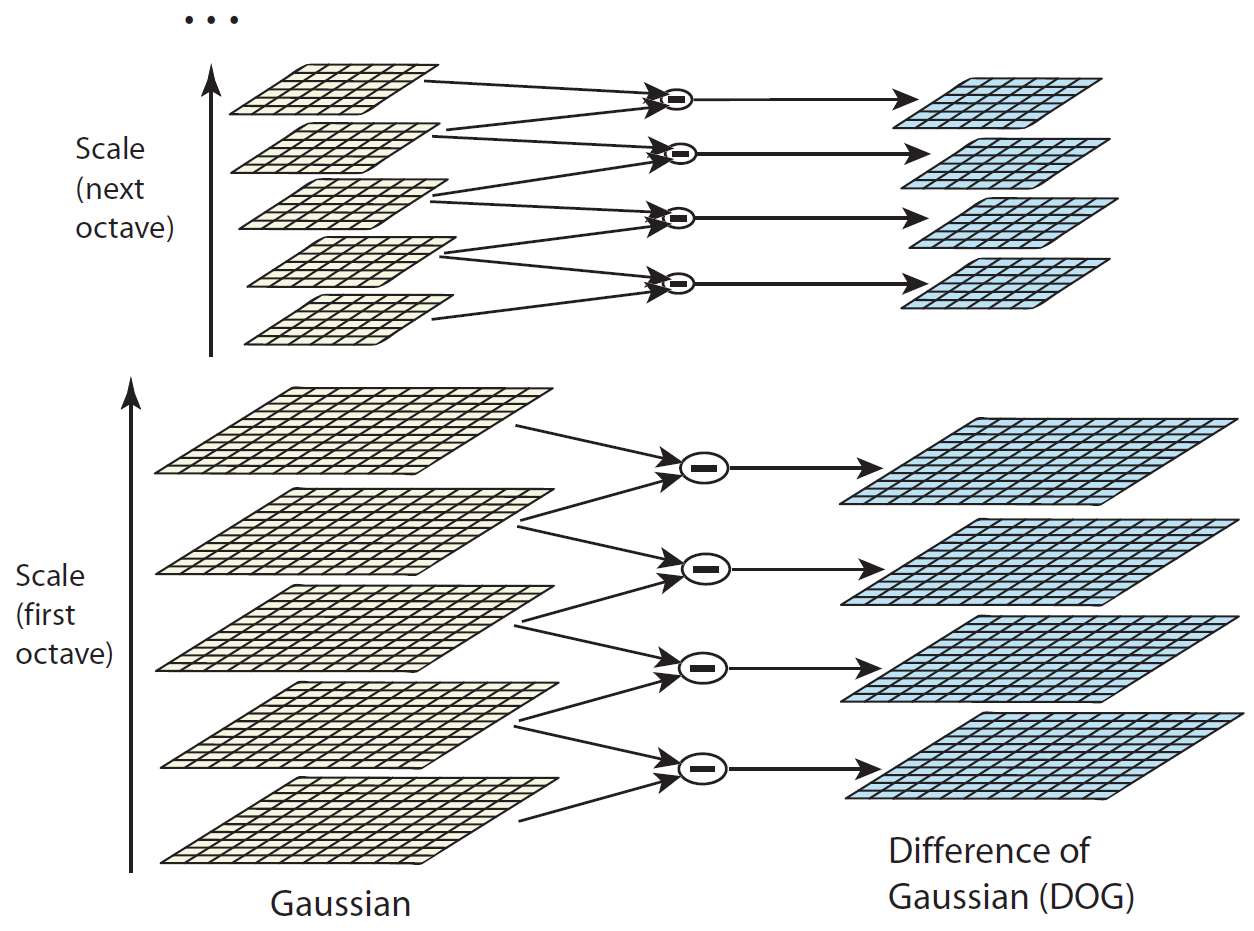
\includegraphics[width=0.8\textwidth]{img/pyramide_gaussienne.png}
    \caption{\textit{Schéma de la pyramide gaussienne et des différences de gaussiennes (DoG). Extrait de la documentation OpenCV sur l'implémentation SIFT.}}
    \label{fig:pyramide_gaussienne}
\end{figure}

\section{Localisation précise des points clés}

Une fois les images DoG générées, l'algorithme cherche les extremums locaux. Un pixel est considéré comme un candidat s'il est strictement supérieur (ou strictement inférieur) à ses 8 voisins dans l'image courante, ainsi qu'à ses 9 voisins dans l'échelle supérieure et ses 9 voisins dans l'échelle inférieure (soit 26 voisins au total).

Cependant, cette détection brute produit beaucoup de points erronés ou mal localisés.

\begin{figure}[h]
    \centering
    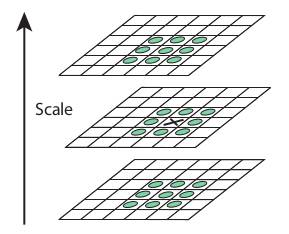
\includegraphics[width=0.8\textwidth]{img/sift_local_extrema.jpg}
    \caption{\textit{Illustration de la détection des extremums locaux dans l'espace des échelles. Extrait de la documentation OpenCV sur l'implémentation SIFT.}}
    \label{fig:sift_local_extrema}
\end{figure}

\subsection{Raffinement Sub-pixel (Interpolation de Taylor)}
Les extremums détectés sont initialement positionnés sur la grille discrète des pixels. Pour une précision sub-pixel (nécessaire pour un matching précis), SIFT modélise la fonction DoG localement par un développement de Taylor du second ordre :

\begin{equation}
    D(\mathbf{x}) = D + \frac{\partial D}{\partial \mathbf{x}}^T\mathbf{x} + \frac{1}{2}\mathbf{x}^T \frac{\partial^2 D}{\partial \mathbf{x}^2}\mathbf{x}
\end{equation}

où $\mathbf{x} = (x, y, \sigma)^T$ est le décalage par rapport au point d'échantillonnage. La position exacte de l'extremum $\hat{\mathbf{x}}$ est trouvée en annulant la dérivée de cette fonction par rapport à $\mathbf{x}$ :
\begin{equation}
    \hat{\mathbf{x}} = - \left( \frac{\partial^2 D}{\partial \mathbf{x}^2} \right)^{-1} \frac{\partial D}{\partial \mathbf{x}}
\end{equation}

Si le décalage calculé $\hat{\mathbf{x}}$ est supérieur à 0.5 dans une direction, le point d'interpolation se trouve plus près d'un voisin : l'algorithme déplace alors le point central et réitère le calcul.

\subsection{Filtrage des points à faible contraste}
Les points situés dans des zones homogènes sont sensibles au bruit. On évalue la valeur de la fonction DoG au point interpolé $D(\hat{\mathbf{x}})$. Si cette valeur est trop faible (typiquement $|D(\hat{\mathbf{x}})| < 0.03$ pour des pixels normalisés entre 0 et 1), le point est rejeté.

\subsection{Élimination des réponses de bords}
C'est une étape cruciale. La fonction DoG réagit fortement sur les arêtes (bords), tout comme un détecteur de contours. Or, un point situé sur une ligne droite est mal localisé dans la direction de la ligne (problème d'ouverture). On veut conserver uniquement les "coins" ou les "taches".

Pour cela, on analyse la courbure principale via la matrice Hessienne $2\times2$, $H$, calculée au point clé :
\begin{equation}
    H = \begin{bmatrix} D_{xx} & D_{xy} \\ D_{xy} & D_{yy} \end{bmatrix}
\end{equation}

Les valeurs propres de $H$ sont proportionnelles aux courbures principales. Plutôt que de calculer explicitement ces valeurs propres, SIFT utilise une astuce algébrique basée sur la trace ($Tr(H) = D_{xx} + D_{yy}$) et le déterminant ($Det(H) = D_{xx}D_{yy} - (D_{xy})^2$).
Pour rejeter les arêtes, on vérifie si le rapport des courbures principales est inférieur à un seuil $r$ (Lowe utilise $r=10$) via la condition suivante :

\begin{equation}
    \frac{\text{Tr}(H)^2}{\text{Det}(H)} < \frac{(r+1)^2}{r}
\end{equation}

Si cette inégalité n'est pas vérifiée, cela signifie que la courbure est très forte dans une direction et faible dans l'autre (cas typique d'une arête) : le point est alors supprimé.

\section{Assignation d'orientation}
À ce stade, nous avons des points stables ($\mathbf{x}$) à une échelle précise ($\sigma$). Pour rendre le descripteur invariant à la rotation de l'image, on attribue une orientation canonique à chaque point clé.

\begin{figure}[h]
    \centering
    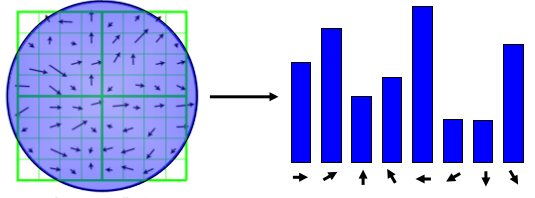
\includegraphics[width=0.6\textwidth]{img/orientation.png}
    \caption{\textit{Calcul de l'orientation principale autour du point clé. Extrait de l'étude de Liu et al. (2008).}}
    \label{fig:sift_orientation}
\end{figure}

Les calculs sont effectués sur l'image gaussienne $L$ la plus proche de l'échelle du point clé, afin que les calculs de gradients soient cohérents avec le niveau de flou de la structure détectée.
Pour chaque pixel $(x,y)$ dans un voisinage autour du point clé, on calcule la magnitude $m(x,y)$ et l'orientation $\theta(x,y)$ du gradient :

\begin{equation}
    m(x,y) = \sqrt{(L_{x+1,y} - L_{x-1,y})^2 + (L_{x,y+1} - L_{x,y-1})^2}
\end{equation}
\begin{equation}
    \theta(x,y) = \tan^{-1}\left(\frac{L_{x,y+1} - L_{x,y-1}}{L_{x+1,y} - L_{x-1,y}}\right)
\end{equation}

Un histogramme d'orientation à 36 bins (couvrant les 360 degrés) est construit. Chaque échantillon ajouté à l'histogramme est pondéré par :
\begin{enumerate}
    \item Sa magnitude $m(x,y)$.
    \item Une fenêtre gaussienne circulaire centrée sur le point clé (avec $\sigma_{win} = 1.5 \times \sigma_{keypoint}$), pour donner plus d'importance aux gradients proches du centre.
\end{enumerate}

Le pic le plus haut de l'histogramme définit l'orientation principale. Si des pics secondaires dépassent 80\% de la hauteur du pic principal, un nouveau point clé est créé au même endroit et à la même échelle, mais avec cette orientation secondaire. Cela permet à SIFT de gérer de manière robuste les coins ambigus.

\section{Descripteur de point clé}
La dernière étape consiste à calculer une empreinte numérique (le descripteur) qui soit très distinctive tout en restant robuste aux variations locales (petits changements de perspective, illumination).

\begin{figure}[h]
    \centering
    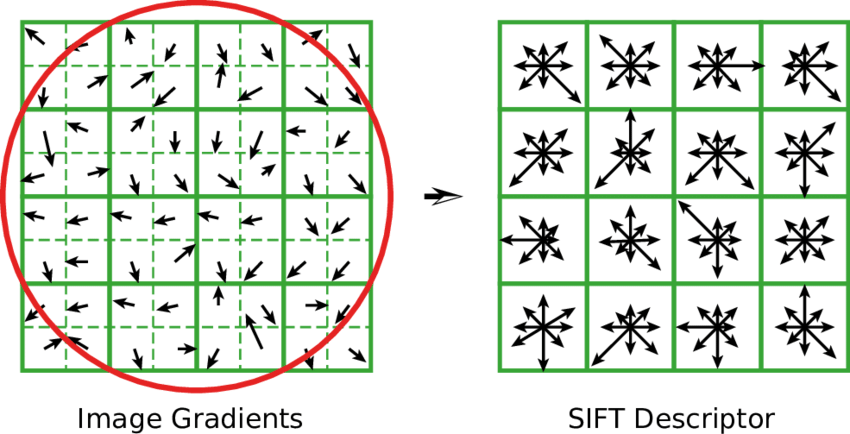
\includegraphics[width=0.7\textwidth]{img/SIFT-descriptor-The-well-known-SIFT-descriptor-consists-of-3D-histograms-of-image.png}
    \caption{\textit{Construction du descripteur SIFT à partir des histogrammes de gradients locaux. Extrait de la documentation OpenCV sur l'implémentation SIFT.}}
    \label{fig:sift_descriptor}
\end{figure}
\subsection{Construction de la grille}
On considère une région carrée autour du point clé. \textbf{Point crucial :} cette région est orientée selon l'angle principal calculé à l'étape précédente. C'est cette rotation du système de coordonnées qui garantit l'invariance par rotation.

La région est divisée en une grille de $4 \times 4$ sous-régions. Dans chaque sous-région, on compile un histogramme d'orientation sur 8 directions (points cardinaux et inter-cardinaux).
Afin d'éviter les effets de frontières brusques (quand un gradient passe d'une sous-région à l'autre), la contribution de chaque pixel est distribuée par interpolation trilinéaire (sur x, y et l'angle $\theta$).

\subsection{Le vecteur final et sa normalisation}
Le descripteur final est la concaténation de ces histogrammes :
$$ 4 \times 4 \text{ sous-régions } \times 8 \text{ orientations } = 128 \text{ dimensions} $$

Ce vecteur $v$ subit enfin une procédure de normalisation pour l'invariance photométrique :
\begin{enumerate}
    \item \textbf{Normalisation unitaire :} $v \leftarrow v / ||v||$. Cela compense les changements linéaires de contraste (gain global).
    \item \textbf{Seuillage :} Les valeurs du vecteur supérieures à 0.2 sont plafonnées à 0.2. Cela réduit l'influence des effets d'illumination non-linéaires (comme les reflets spéculaires ou la saturation de la caméra).
    \item \textbf{Renormalisation :} Le vecteur est à nouveau normalisé à une longueur unitaire.
\end{enumerate}

Le résultat est un vecteur de 128 flottants, prêt à être comparé par distance Euclidienne pour le matching.

\chapter{Analyse et Discussion des Résultats}

Au-delà de l'implémentation technique, il est essentiel d'analyser pourquoi SIFT est devenu un standard industriel pendant deux décennies, mais aussi de comprendre les contraintes qui ont mené au développement de méthodes alternatives (comme SURF ou ORB).

\section{Analyse de la Robustesse (Avantages)}

L'avantage majeur de SIFT réside dans la "distinctivité" de ses descripteurs. Là où des méthodes plus anciennes se contentaient de corréler des zones de pixels (sensibles aux changements d'intensité), SIFT transforme l'information locale en une signature vectorielle de haute dimension.

\subsection{Invariances Géométriques}
\begin{itemize}
    \item \textbf{Invariance d'Échelle et de Rotation :} C'est la promesse centrale de l'algorithme. Grâce à l'espace des échelles (pyramide gaussienne) et à l'assignation d'une orientation canonique, un objet peut être reconnu même s'il apparaît 5 fois plus petit ou s'il a subi une rotation quelconque.
    \item \textbf{Robustesse aux déformations affines :} Bien que SIFT ne modélise pas explicitement les transformations affines complètes (étirement, cisaillement), Lowe a démontré expérimentalement que les descripteurs restent robustes pour des changements de point de vue allant jusqu'à 50 degrés. Au-delà, la déformation des motifs locaux devient trop importante pour que les histogrammes de gradients restent corrélés.
\end{itemize}

\subsection{Invariance Photométrique}
Notre étude du descripteur a montré que SIFT est particulièrement résistant aux variations d'éclairage, grâce à une stratégie de normalisation en deux temps :
\begin{enumerate}
    \item \textbf{Changement linéaire (Contraste/Luminosité) :} La normalisation du vecteur descripteur à une longueur unitaire ($||v||=1$) annule les changements multiplicatifs d'intensité.
    \item \textbf{Saturation non-linéaire :} En plafonnant les valeurs du vecteur à 0.2, SIFT réduit l'impact des effets non-linéaires importants, comme les reflets spéculaires ou la saturation du capteur de la caméra.
\end{enumerate}

\subsection{Discrimination (Matching)}
La dimensionnalité élevée (128) du vecteur permet une discrimination très fine. Lowe suggère d'utiliser le rapport de distance ($L_2$) entre le plus proche voisin et le second plus proche voisin (NNDR - \textit{Nearest Neighbor Distance Ratio}). Si ce ratio est inférieur à 0.8, le match est considéré comme valide. Cette méthode permet d'éliminer plus de 90\% des faux positifs tout en conservant plus de 95\% des correspondances correctes.

\section{Limites Intrinsèques de la Méthode}

Malgré ses performances, notre implémentation et la littérature mettent en évidence plusieurs goulots d'étranglement.

\subsection{Coût de Calcul et Complexité}
SIFT est un algorithme lourd.
\begin{itemize}
    \item \textbf{Construction de l'espace des échelles :} La nécessité de réaliser de nombreuses convolutions gaussiennes et soustractions sur plusieurs octaves est coûteuse en temps CPU.
    \item \textbf{Dimension du descripteur :} Le vecteur de 128 flottants est lourd à stocker et à comparer. Dans une base de données contenant des milliers d'images, la recherche des plus proches voisins (même avec des structures optimisées comme les arbres k-d) reste une opération critique. C'est ce qui a motivé la création de descripteurs binaires comme BRIEF ou ORB, beaucoup plus rapides à comparer via la distance de Hamming.
\end{itemize}

\subsection{Le problème des zones peu texturées}
Comme nous l'avons observé sur l'image "Cameraman", SIFT dépend de la présence de gradients locaux.
\begin{itemize}
    \item \textbf{Zones uniformes :} Le ciel ou les surfaces lisses ne génèrent pas d'extremums dans la différence de Gaussiennes.
    \item \textbf{Problème d'ouverture :} Bien que le rejet des arêtes (via la Hessienne) soit efficace, il signifie que SIFT ne peut pas exploiter les contours rectilignes (comme les bords d'un bâtiment) pour le matching, se limitant aux coins et aux taches texturées.
\end{itemize}

\subsection{Invariance Affine Limitée}
SIFT approxime les régions d'intérêt par des cercles. Lorsque la caméra change d'angle de vue de manière drastique (vue rasante), ces cercles devraient idéalement devenir des ellipses. SIFT ne compensant pas cette déformation elliptique, la performance chute drastiquement au-delà de 50 à 60 degrés d'angle. Des extensions comme \textit{ASIFT (Affine-SIFT)} résolvent ce problème en simulant toutes les vues affines possibles, mais au prix d'une explosion du temps de calcul.

\chapter{Implémentation Détaillée}

Dans ce chapitre, vous retourverez la façon dont nous avons implémenté les 3 premières étapes de SIFT (à la demande de notre professeur, Monsieur R.Condat). Nous avons fait le choix de développer l'algorithme en Python en limitant l'usage de bibliothèques externes.
\begin{itemize}
    \item \textbf{Numpy :} Utilisé pour toutes les opérations matricielles (algèbre linéaire, calculs de gradients, histogrammes).
    \item \textbf{OpenCV (cv2) :} Utilisé strictement pour les opérations de bas niveau (chargement d'image, redimensionnement, et flou gaussien basique), afin de ne pas réinventer la convolution.
    \item \textbf{Matplotlib :} Pour la visualisation des résultats intermédiaires.
\end{itemize}

\section{1. Construction de l'Espace des Échelles (Scale-Space)}

La première étape consiste à générer la pyramide d'images. Dans notre code, cela est géré par la fonction \texttt{build\_gaussian\_octaves}.

\subsection{Génération des sigmas}
Pour chaque octave, nous devons générer une série d'images floutées. Comme spécifié dans la théorie, le facteur multiplicatif entre deux échelles est $k = 2^{1/s}$.
La fonction \texttt{build\_gaussian\_kernels} pré-calcule les valeurs de $\sigma$ nécessaires.

\begin{lstlisting}[language=Python, caption=Calcul des sigmas pour une octave]
def build_gaussian_kernels(sigma, num_scales):
    k = 2 ** (1.0 / num_scales)
    gaussian_kernels = np.zeros(num_scales + 3)
    gaussian_kernels[0] = sigma
    
    for i in range(1, num_scales + 3):
        # Calcul du sigma du noyau à appliquer pour passer de l'image précédente à la suivante
        sigma_prev = (k ** (i - 1)) * sigma
        sigma_total = k * sigma_prev
        gaussian_kernels[i] = np.sqrt(sigma_total ** 2 - sigma_prev ** 2)
        
    return gaussian_kernels
\end{lstlisting}

\subsection{Création des DoG}
La fonction \texttt{generateDoGImages} prend une octave (une liste d'images gaussiennes) et calcule les différences pixel à pixel entre images adjacentes. C'est ici que l'approximation du Laplacien est réalisée.

\begin{lstlisting}[language=Python, caption=Calcul des Différences de Gaussiennes]
def generateDoGImages(gaussian_images):
    dog_images = []
    for i in range(len(gaussian_images) - 1):
        # Soustraction simple des matrices numpy
        dog_images.append(gaussian_images[i+1] - gaussian_images[i])
    return dog_images
\end{lstlisting}

\subsection{Détection des Extremums Locaux}

L'étape de recherche brute est implémentée dans la fonction \texttt{detect\_keypoints\_in\_dog}. Nous itérons sur chaque octave, puis sur chaque échelle $s$ (de 1 à $s-1$), et enfin sur chaque pixel $(i, j)$ de l'image (en excluant les bords pour éviter les erreurs d'index).

La fonction critique est \texttt{is\_extremum}, qui vérifie si un pixel est strictement supérieur ou strictement inférieur à ses 26 voisins :
\begin{itemize}
    \item 8 voisins dans l'échelle courante ($s$).
    \item 9 voisins dans l'échelle inférieure ($s-1$).
    \item 9 voisins dans l'échelle supérieure ($s+1$).
\end{itemize}

\begin{lstlisting}[language=Python, caption=Vérification des 26 voisins]
def is_extremum(first_subimage, second_subimage, third_subimage, threshold):
    center_pixel_val = second_subimage[1, 1]
    
    # Seuil préliminaire pour gagner du temps (si le point est trop faible, on l'ignore)
    if abs(center_pixel_val) < threshold:
        return False

    # Comparaison avec les 26 voisins
    # (Combinaison des 3 sous-blocs 3x3)
    if center_pixel_val > 0:
        return np.all(center_pixel_val >= first_subimage) and \
               np.all(center_pixel_val >= third_subimage) and \
               np.all(center_pixel_val >= second_subimage)
    # ... (idem pour le cas < 0)
\end{lstlisting}

\section{2. Raffinement et Filtrage (Keypoint Localization)}

C'est la partie la plus mathématique de l'implémentation. Nous avons codé les dérivées partielles à l'aide de différences finies centrales.

\subsection{Calcul des Gradients et de la Hessienne}
Pour localiser le point avec une précision sub-pixel, nous avons besoin du gradient $\frac{\partial D}{\partial \mathbf{x}}$ et de la Hessienne $\frac{\partial^2 D}{\partial \mathbf{x}^2}$.
Nous avons implémenté ces calculs manuellement :

\begin{lstlisting}[language=Python, caption=Approximation des dérivées par différences finies]
def compute_gradient_at_center(pixel_array):
    # dx = (f(x+1) - f(x-1)) / 2
    dx = 0.5 * (pixel_array[1, 1, 2] - pixel_array[1, 1, 0])
    dy = 0.5 * (pixel_array[1, 2, 1] - pixel_array[1, 0, 1])
    ds = 0.5 * (pixel_array[2, 1, 1] - pixel_array[0, 1, 1])
    return np.array([dx, dy, ds])

def compute_hessian_at_center(pixel_array):
    center_val = pixel_array[1, 1, 1]
    # dxx = f(x+1) - 2f(x) + f(x-1)
    dxx = pixel_array[1, 1, 2] - 2 * center_val + pixel_array[1, 1, 0]
    dyy = pixel_array[1, 2, 1] - 2 * center_val + pixel_array[1, 0, 1]
    dss = pixel_array[2, 1, 1] - 2 * center_val + pixel_array[0, 1, 1]
    # ... (calcul des dérivées croisées dxy, dxs, dys)
    return np.array([[dxx, dxy, dxs], [dxy, dyy, dys], [dxs, dys, dss]])
\end{lstlisting}

\subsection{Boucle de Raffinement (Newton-Raphson)}
La fonction \texttt{localize\_keypoint} tente de converger vers la position réelle de l'extremum. Elle résout itérativement le système $\mathbf{\hat{x}} = -H^{-1} \nabla D$. Si le décalage calculé est supérieur à 0.5 pixel dans une direction, le centre de la fenêtre est déplacé. Si l'algorithme ne converge pas après 5 itérations, le point est rejeté.

\subsection{Filtrage des Arêtes (Edge Response)}
Une fois le point localisé, nous appliquons le critère de la Hessienne 2x2 (seulement spatiale $x,y$) pour éliminer les arêtes.
\begin{lstlisting}[language=Python, caption=Rejet des arêtes via Trace et Déterminant]
# Hessienne xy seulement
H_xy = hessian[:2, :2]
trace_H = np.trace(H_xy)
det_H = np.linalg.det(H_xy)

# Condition de ratio (r=10 par défaut)
if det_H <= 0 or (trace_H ** 2) / det_H >= ((r + 1) ** 2) / r:
    return None # Point rejeté (c'est une arête)
\end{lstlisting}

\section{3. Assignation d'Orientation}

Pour chaque point clé validé, nous calculons son orientation dominante.

\subsection{Calcul de l'histogramme}
La fonction \texttt{compute\_orientation\_histogram} explore une fenêtre autour du point clé. La taille de cette fenêtre dépend de l'échelle du point clé ($radius = 3 \times 1.5 \times \sigma$).
Pour chaque pixel de cette fenêtre, nous calculons la magnitude et l'orientation du gradient :

\begin{lstlisting}[language=Python, caption=Calcul Magnitude et Orientation]
# Calcul vectorisé numpy
dx = L[y, x+1] - L[y, x-1]
dy = L[y+1, x] - L[y-1, x]
magnitude = np.sqrt(dx**2 + dy**2)
orientation = np.rad2deg(np.arctan2(dy, dx)) % 360
\end{lstlisting}

Ces valeurs remplissent un histogramme de 36 bins (10 degrés par bin), pondéré par une gaussienne centrée sur le point clé.

\subsection{Lissage et Pics}
L'histogramme brut est lissé (fonction \texttt{smooth\_histogram}) pour réduire le bruit. Enfin, la fonction \texttt{assign\_orientations} identifie le pic maximal. Si des pics secondaires dépassent 80\% du pic maximal, nous dupliquons le point clé avec cette nouvelle orientation, ce qui améliore la robustesse de la détection.

\section{Structure des données de sortie}
À la fin du pipeline, nos points clés sont stockés sous forme d'objets \texttt{cv2.KeyPoint}. Cela nous permet d'utiliser la fonction \texttt{cv2.drawKeypoints} pour visualiser facilement nos résultats et comparer notre implémentation "maison" avec celle d'OpenCV.

\begin{lstlisting}[language=Python, caption=Création de l'objet KeyPoint final]
new_kp = cv2.KeyPoint()
new_kp.pt = tuple(position_reelle * (2 ** octave_index)) # Remise à l'échelle originale
new_kp.size = sigma * (2 ** (octave_index + 1))
new_kp.angle = peak_angle
new_kp.response = abs(extremum_val)
keypoints.append(new_kp)
\end{lstlisting}

\chapter{Conclusion}
Le projet nous a permis de décortiquer l'algorithme SIFT. En passant de la théorie mathématique (espace des échelles, Hessienne) à l'implémentation pratique en Python, nous avons pu constater la finesse de la méthode proposée par Lowe. La combinaison d'une détection multi-échelle et d'une description locale robuste fait de SIFT une pierre angulaire de la vision par ordinateur moderne, malgré l'émergence récente de méthodes basées sur le Deep Learning.

\appendix
\chapter{Références}
\begin{enumerate}
    \item Lowe, D. G. (2004). Distinctive Image Features from Scale-Invariant Keypoints. \textit{International Journal of Computer Vision}.
    \item Support de présentation "Traitement d'image: SIFT", Projet TIM, Louis LENOBLE, Raphael ROGER, Dylan SANSON, Jack SU, 2025.
    \item Documentation OpenCV sur l'implémentation SIFT : \url{https://docs.opencv.org/4.x/da/df5/tutorial_py_sift_intro.html}
    \item Liu, C., Yuen, J., & Torralba, A. (2008). SIFT Flow: Dense Correspondence across Different Scenes. \textit{IEEE Transactions on Pattern Analysis and Machine Intelligence}.
    \item Wikipedia - Scale-invariant feature transform: \url{https://fr.wikipedia.org/wiki/Scale-invariant_feature_transform}
\end{enumerate}

\end{document}